\chapter{\IfLanguageName{dutch}{Analyse van de cijfers}{Analysis of the figures}}%
\label{ch:analyse}

Allereerst heeft er een online vragenlijst plaatsgevonden. Daarna is de POC in gebruik genomen door diezelfde mensen als zij die de vragenlijst ingevuld hebben. Tenslotte is nogmaals een vragenlijst uitgestuurd om eventuele veranderingen of evoluties op te merken.

De twintig bevraagde mensen zijn allen werkzaam in een sedentaire job. 45\% van de respondenten zijn tussen de 18 en 25 jaar oud, 40\% tussen de 25 en 35 jaar oud en de overige 15\% zijn tussen de 35 en 45 jaar oud. Deze bachelorproef kan dus geen conclusies trekken over mensen die zich buiten deze leeftijdsgroepen bevinden.

\section{Resultaten voor gebruik van Move-it!}

\subsection{Beweging}
Slechts 30\% van de bevraagde personen is tevreden met diens hoeveelheid dagelijkse beweging (figuur \ref{fig:dagelijkseBeweging}).

\begin{figure}[h]
    \caption[In welke mate vindt u van uzelf dat u dagelijks voldoende beweegt (op een schaal van 1 tot en met 5)?]{In welke mate vindt u van uzelf dat u dagelijks voldoende beweegt (op een schaal van 1 tot en met 5)?}
    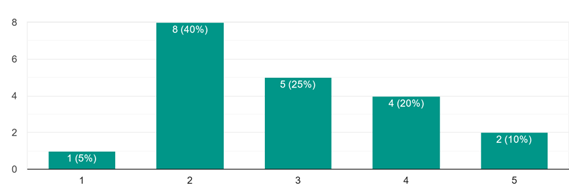
\includegraphics[width=1\textwidth]{DailyMovement}
    \label{fig:dagelijkseBeweging}
\end{figure}

Volgens de WHO moeten volwassenen tussen de 18 en 64 jaar oud wekelijks ongeveer 150 à 300 minuten met gemiddelde intensiteit sporten. % TODO: bron
Uit dit onderzoek is gebleken dat 45\% van de 18 à 45 jaar oude mensen dit voorgeschreven aantal niet halen. 20\% van hen sport meer dan 5 uur per week met gemiddelde intensiteit. Dit wil zeggen dat slechts 35\% van de mensen dit aangeraden aantal behaalt.

WHO stelt dat volwassenen van diezelfde leeftijdsgroep ongeveer 75 à 150 minuten met hoge intensiteit moeten sporten. % TODO: bron
50\% van de respondenten behaalt dit doel en 35\% van hen doet zelfs meer dan de aangeraden 150 minuten.

\subsection{Motivatie}

\begin{figure}[h]
    \caption[Zou u liever meer sporten dan u op dit moment doet?]{Zou u liever meer sporten dan u op dit moment doet?}
    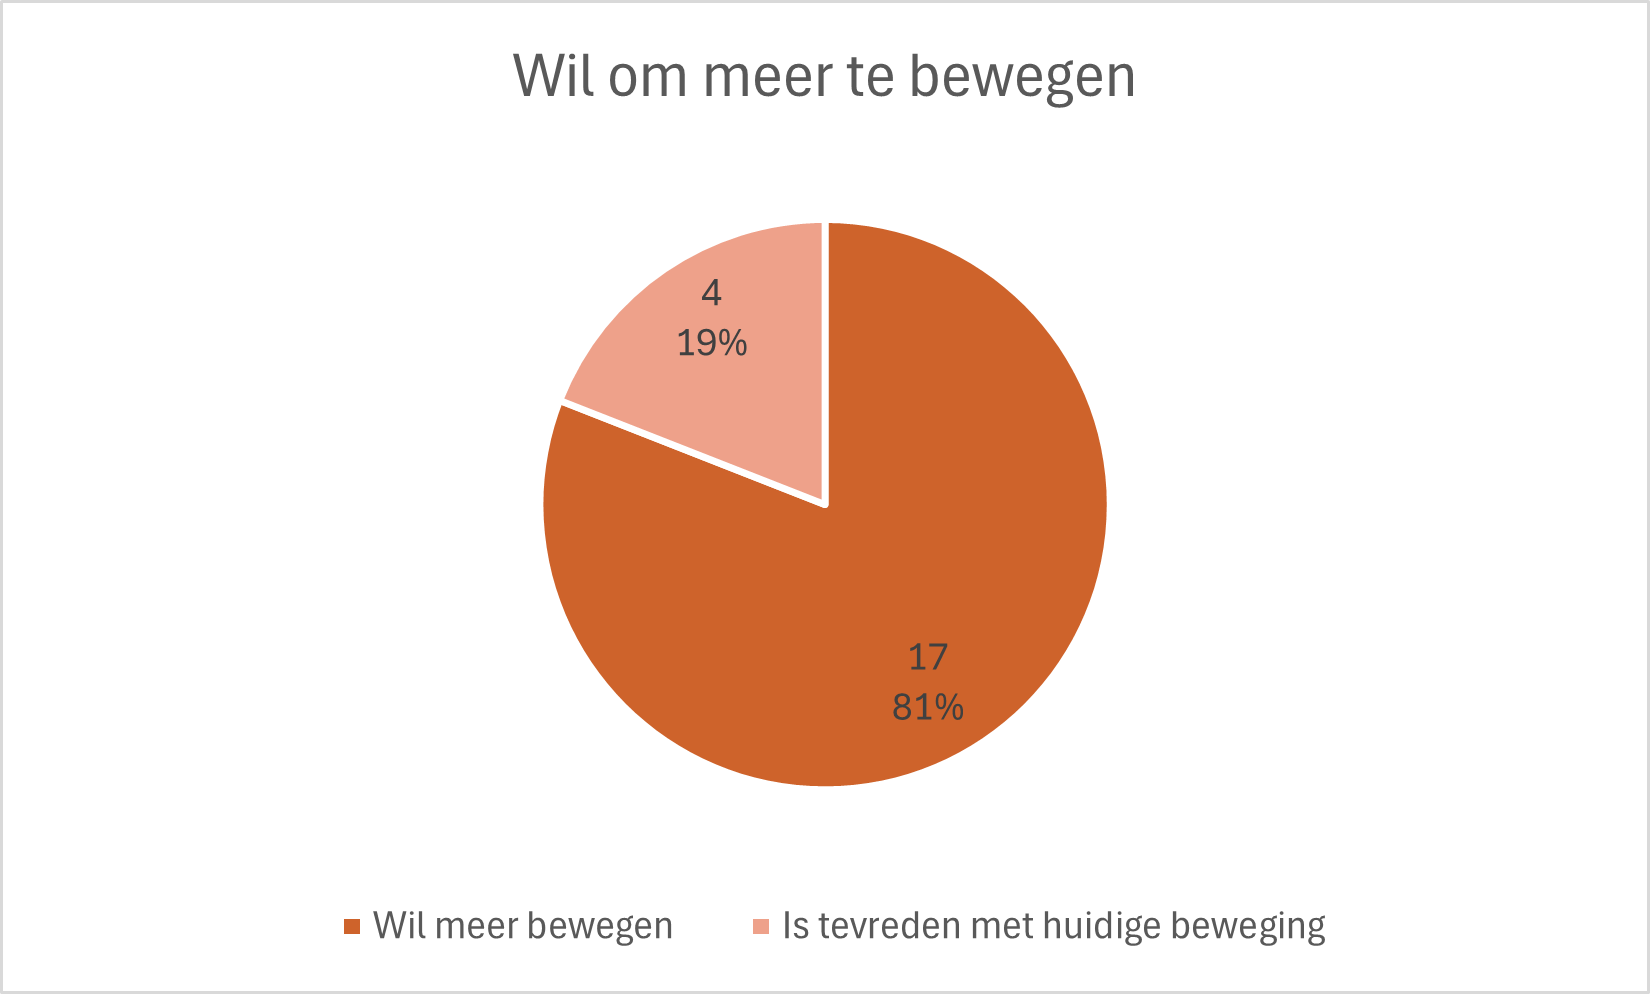
\includegraphics[width=1\textwidth]{MeerSporten}
    \label{fig:meerBewegen}
\end{figure}

Slechts drie van de twintig mensen zijn tevreden met de hoeveelheid sport die ze op dit moment doen. Ruim 85\% is dus niet tevreden en zou liever meer sporten dan die op dit moment doet (figuur \ref{fig:meerBewegen}).

Het grootste probleem voor mensen om meer te sporten, is tijd vinden. Daarnaast staan ook motivatie en wederkerende blessures in de weg. Een minderheid vindt ook geen plezier in het sporten (figuur \ref{fig:waarom}).

\begin{figure}[h]
    \caption[Wat houdt u op dit moment tegen om meer te sporten?]{[Wat houdt u op dit moment tegen om meer te sporten?}
    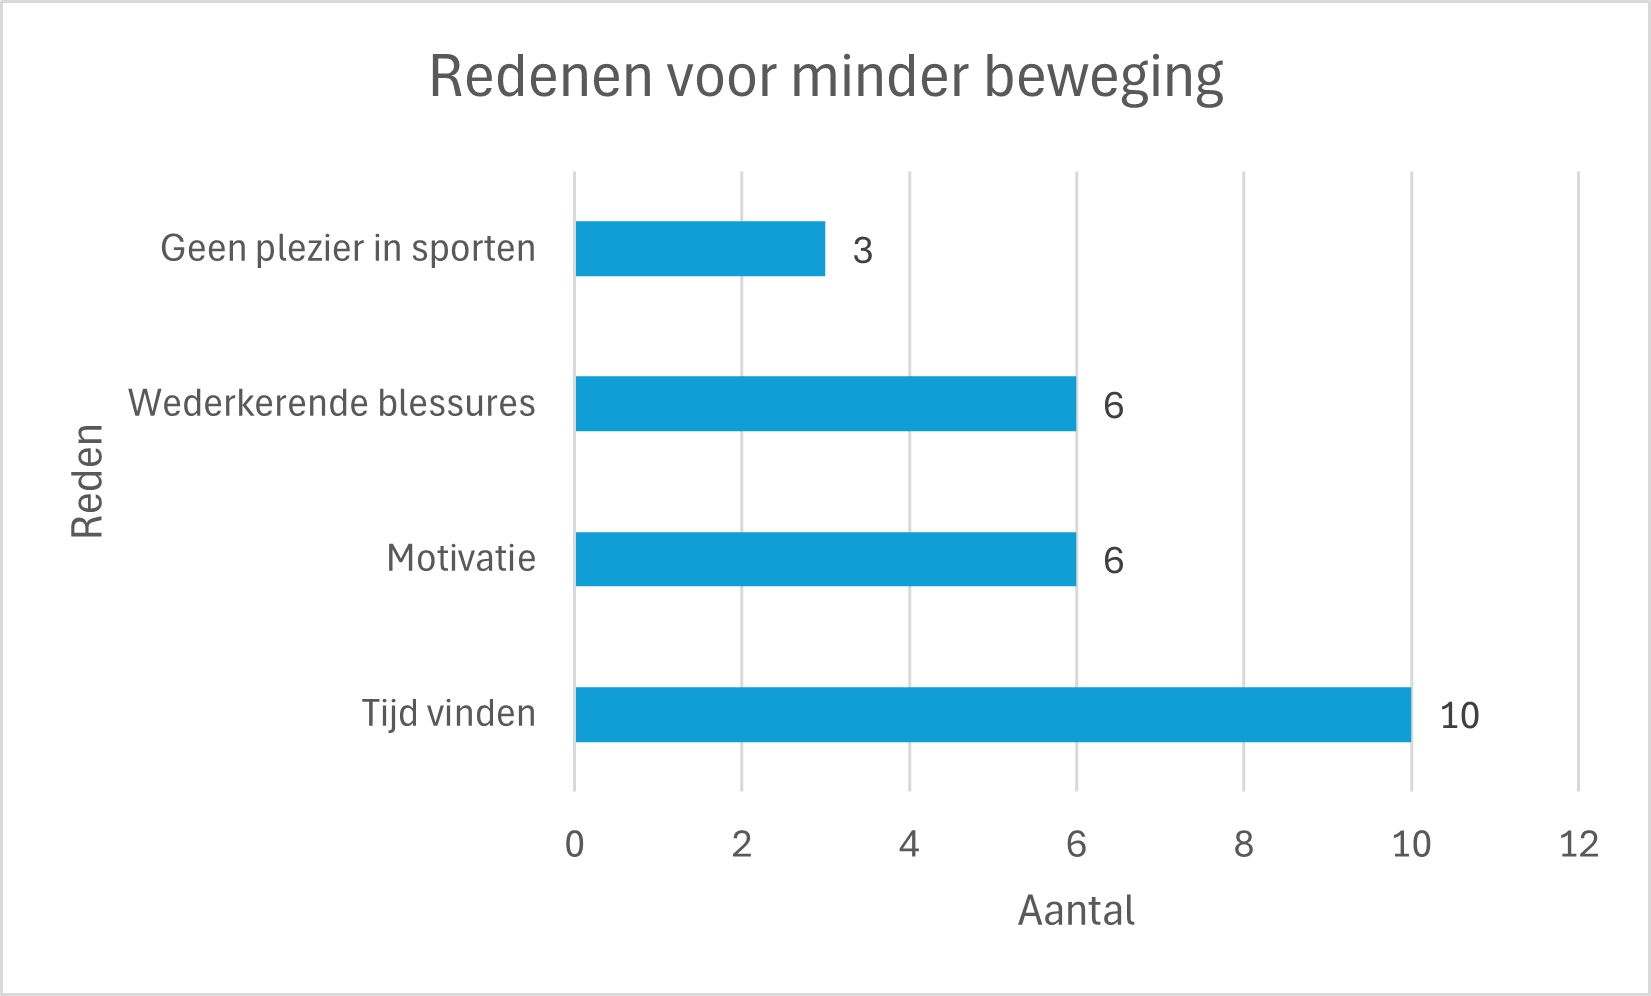
\includegraphics[width=1\textwidth]{Waarom}
    \label{fig:waarom}
\end{figure}

\subsection{Gamification}

Grote voorkeur voor focus op persoonlijke vooruitgang: feature die in Strava betalend is...

Gamification wordt eigenlijk niet zo vaak als vervelend ervaren

Wat wel als vervelend wordt ervaren zijn meldingen en sociale interacties (zoals likes ed)

\section{Sportresultaten}

Evolutie meten. Hoeveel percent haalt de voorgeschreven hoeveelheden.

\section{Resultaten na gebruik van Move-it!}

Nieuwe vragenlijst maken!

- focus op gevoel
- meer sporten in de toekomst?
- wat was anders dan andere sportapplicaties?
    - was dit beter of slechter?
- als u 1 ding zou kunnen veranderen, wat?